% !Mode:: "TeX:UTF-8"
\documentclass[aspectratio=169, 12pt, utf8, mathserif]{ctexbeamer} %aspectratio=43 or aspectratio=169
%%%%%%%%%%%%%%%%%%%%%%%%%%%%%%%%%%%%%%%%%%%%%%%%%%%%%%%%%%%%%%%%%%%%%%%%%%%%%%%%%%%%%%%%%%%%%%%%%%%%%%%%%%%%%%%%%%%%%%%%%%%%%%%%%%%%%%%%%%%%%%%%%%%%%%%%
%-----------------导言区-----------------------------------------------------------
\usepackage{ctex} %加载中文字体
%\usepackage{xeCJK}
\usepackage{amsmath, amsfonts, amssymb, amsthm, mathtools} %加载数学公式
\usepackage{graphicx} %加载图形宏包
\usepackage{fontspec} %加载字体宏包
\usepackage{tikz} %加载绘图TikZ
\usepackage{ulem} %解决下划线换行紊乱
\usepackage{booktabs} %表格功能包
\usepackage{multirow} %合并多行表格
\usepackage{caption} %添加标题
\usepackage{subfigure} %加载子图宏包
\usepackage{theorem} %加载数学定理宏包
\usepackage[style=gb7714-2015]{biblatex} %加载GB7714参考文献样式
%\usepackage[backend=bibtex,style=numeric-comp,sorting=none]{biblatex} %不列出所有作者
%\usepackage[backend=bibtex,sorting=none,maxnames=9,minnames=3]{biblatex} %列出所有作者
%\addbibresource{ref.bib} %BibTeX数据文件及位置
\setbeamerfont{footnote}{size=\tiny} %设置脚注引用文献的字体大小
\setbeamertemplate{bibliography item}[text] %设置参考文献图标样式数字标号
\usepackage{multicol} %分栏
\usepackage[marginal]{footmisc} %首页添加脚注无缩进
\renewcommand{\thefootnote}{} %首页添加脚注无编号
\usepackage{enumerate} %加载列表宏包
\usepackage{wallpaper} %添加水印
\usepackage{listings} %代码包
\usepackage{xcolor} %代码高亮包
\usepackage{hyperref} %正文区
\usepackage{textpos} %导言部分加载 textpos 宏包
\usepackage{booktabs}
\usepackage{media9} %插入视频



%-----------------------设置模板--------------------------------
%\setbeamertemplate{navigation symbols}{} %取消导航
%\setCJKmainfont{SimHei} %中文用黑体
%\setmainfont{Times New Roman} %英文字体
%\setmonofont{Consolas} %代码字体和学号字体
\setbeamertemplate{caption}[numbered] %显示图表的标号
\setlength{\abovecaptionskip}{0.cm}	%设置表格题注的上间距
\setlength{\belowcaptionskip}{-0.08cm} %设置表格题注的下间距

%-------------------设置颜色、外框颜色等------------------------
\useinnertheme{circles}
\useoutertheme{infolines} %适用于上课和组会等汇报的主题
\usecolortheme{crane} % 罗列环境的色调符合
\usefonttheme{default}
\usefonttheme{professionalfonts}
%\usefonttheme{serif}
%\usefonttheme{structurebold}
%\usefonttheme{structureitalicserif}

\setbeamertemplate{blocks}[rounded]

%----------------------设置页脚格式------------------------------
\setbeamertemplate{footline}
{
	\leavevmode
	\hbox
	{
		\begin{beamercolorbox}[wd=0.3\paperwidth,ht=2.8ex,dp=1ex,center]{author in head/foot}
			\usebeamerfont{author in head/foot} \insertshortauthor \quad \insertshortinstitute
		\end{beamercolorbox}
		\begin{beamercolorbox}[wd=0.4\paperwidth,ht=2.8ex,dp=1ex,center]{title in head/foot}
			\usebeamerfont{title in head/foot}\insertshorttitle
		\end{beamercolorbox}
		\begin{beamercolorbox}[wd=0.3\paperwidth,ht=2.8ex,dp=1ex,center]{date in head/foot}
			\usebeamerfont{date in head/foot}\insertshortdate{} \quad
			\insertframenumber{} / \inserttotalframenumber
		\end{beamercolorbox}
	}
	\vskip 0pt
}



%-----------------------定义颜色-----------------------------------
\definecolor{blue01}{RGB}{19,63,127} %浅蓝紫色
\definecolor{blue02}{RGB}{0,30,108} %深蓝紫色
\definecolor{blue03}{RGB}{0,87,146} %浅蓝灰色
\definecolor{blue04}{RGB}{3,83,151} %深蓝灰色
\definecolor{red01}{RGB}{192,0,0} %浅砖红色
\definecolor{red02}{RGB}{172,0,0} %深砖红色
\definecolor{red03}{RGB}{210,85,101} %淡红色
\definecolor{gray01}{RGB}{246,248,255} %白灰色
\definecolor{green02}{RGB}{0,107,116} %深绿色
\definecolor{dkgreen}{RGB}{0,153,0} %matlab代码色
\definecolor{gray}{RGB}{128,128,128} %matlab代码色
\definecolor{mauve}{RGB}{153,0,204} %matlab代码色

\definecolor{exampleblockcolor}{RGB}{19,63,127} % 设置exampleblock的背景颜色
\setbeamercolor{block title example}{bg=exampleblockcolor, fg=white} % 设置exampleblock标题的颜色


% 修改编号环境的颜色
\setbeamertemplate{itemize item}{\color{red01}$\bullet$} %无序项目编号的颜色
\setbeamercolor{section number projected}{bg=red02!50!,fg=blue01!150!} %目录编号的颜色
\setbeamercolor{section in toc}{fg=blue01} %目录中一级标题的颜色
\setbeamercolor{subsection in toc}{fg=red02} %目录中一级标题的颜色

% 修改块环境的颜色和字体
\setbeamercolor{block title}{bg=blue01} %标题块的背景色
\setbeamercolor{block body}{bg=white} %内容块的底板
\setbeamercolor{block title}{fg=white} %块标题文字的颜色
\setbeamercolor{block body}{fg=black} %块中内容字体的颜色
\setbeamerfont{block title}{size=\small} %块标题字体大小,\tiny \scriptsize \footnotesize \small \normalsize \large \Large \LARGE \huge \Huge

% infolines模式下的页眉页脚设置
%\setbeamerfont{title}{size=\Large}
%\setbeamercolor{titlelike}{bg=white,fg=red01} %标题页和三级标题
%\setbeamercolor{palette primary}{bg=blue01,fg=white} %页脚右侧和二级标题
%\setbeamercolor{palette secondary}{bg=red03,fg=white} %页脚中间和主题名
%\setbeamercolor{palette tertiary}{bg=blue01,fg=white} % 页脚左侧和一级标题
%\setbeamerfont{frametitle}{shape=\bfseries} %frame标题字体加粗

\setbeamerfont{title}{size=\Large}
\setbeamercolor{titlelike}{bg=white,fg=red01} %标题页和三级标题
\setbeamercolor{palette primary}{bg=blue01,fg=white} %页脚右侧和二级标题
\setbeamercolor{palette secondary}{bg=blue01,fg=white} %页脚中间和主题名
\setbeamercolor{palette tertiary}{bg=blue01,fg=white} % 页脚左侧和一级标题
\setbeamerfont{frametitle}{shape=\bfseries} %frame标题字体加粗

%%%%%%%%%%%%%%%%%%%%%%%%%%%%%%%%%%%%%%%%%%%%%%%%%%%%%%%%%%%%%%%%%%%%%%%%%%%%%%%%%%%%%%%%%%%%%%%%%%%%%%%%%%%%%%%%%%%%%%%%%%%%%%%%%%%%

% 设置用acrobat打开就会全屏显示
\hypersetup{pdfpagemode=FullScreen}

% 设置logo
% \logo{
\includegraphics[width=1cm]{figures/logo}}
% Logo放到frametitle右侧
\setbeamertemplate{frametitle}
{
		\begin{beamercolorbox}[wd=\paperwidth]{frametitle}
				\strut\hspace{0.5em}\insertframetitle\strut
				\hfill
				\raisebox{-3.3mm}{
\includegraphics[width=1.0cm]{figures/logo}} %校标和代码放同个文件夹下
			\end{beamercolorbox}
}

%%%%%%%%%%%%%%%%%%%%%%%%%%%%%%%%%%%%%%%%%%%%%%%%%%%%%%%%%%%%%%%%%%%%%%%%%%%%%%%%%%%%%%%%%%%%%%%%%%%%%%%%%%%%%%%%%%%%%%%%%%%%%%%%%%%%%%%%%%%%

%-------------开始-------------------------------------------------
\begin{document}

% 每个章节都有小目录
\AtBeginSubsection[]
{
 \begin{frame}
			\frametitle{节目录}
			\begin{multicols}{2}
					\tableofcontents[currentsection]
				\end{multicols}
	 \end{frame}
		\addtocounter{framenumber}{-1}
	}

	
%----------------------------第一页-----------------------------	
\title[Week 1 Team Report]{\bf The Supply Chain and Operations Management} %汇报内容标题
\subtitle{\bf \color{blue01} Subtitle of the report} %汇报内容的作者

\author[\href{}{}]
{
	{\songti \zihao{-4}  \bfseries Sijie Li}  \\ \vspace*{0.1cm}
	%{\zihao{5}  \texttt{\today}}
}

\institute[]
{
		School of Economics and Management\\
		Southeast University
}
\date{\today}%可以加上日期,显示位置在每页的右下角
	

\begin{frame}
	\maketitle
	%\titlepage
\end{frame}
	
\section*{Outline}
% \subsection*{CONTENTS}
\begin{frame}
	\frametitle{Outline}
	\tableofcontents
\end{frame}


%------------------第一部分,背景信息------------------------
\section{Background}
\subsection{Research Interests}	
\begin{frame}
	\frametitle{非自组织植被模式}
	\begin{columns}
		\column{0.34\paperwidth}
		\hspace{5cm} % 插入水平空白
		\vspace{-0.5cm} % 插入垂直空白,上下
		\begin{figure}[tbph]
			\centering
			\includegraphics[width=0.7\textwidth]{figures/3}
			\begin{textblock*}{5cm}(0.2cm,0.2cm)
				\small 斑点、条纹等其他植被模式
			\end{textblock*}
		\end{figure}
		
		\vspace{-0.5cm} % 向上移动
		\column{0.5\paperwidth}	
		\begin{figure}[tbph] % 新的图像
			\centering
			\includegraphics[width=0.6\textwidth]{figures/2} % 更改图像文件名和宽度
			\begin{textblock*}{5cm}(1.5cm,0.25cm) % 调整坐标和文本位置
				\small 仙女环植被模式
			\end{textblock*}
		\end{figure}
		
		\end{columns}
\end{frame}

%%%%%%%%%%%%%%%%%%%%%%%%%%%%%%%%%%%%%%%%%%%%%%%%%%%%%%%%%%%%%%
%	
%	\begin{frame}
%		\frametitle{示例视频}
%		
%		% 插入视频
%		\includemedia[
%		width=0.8\linewidth,
%		height=0.6\linewidth,
%		activate=pageopen,
%		addresource=sample.mp4,
%		flashvars={source=sample.mp4}
%		]{}{VPlayer9.swf}
%	\end{frame}
%
%%%%%%%%%%%%%%%%%%%%%%%%%%%%%%%%%%%%%%%%%%%%%%%%%%%%%%%%%%%%%%%


\begin{frame}
	\frametitle{自组织植被模式}
	\begin{columns}
		\column{0.5\paperwidth} % 调整列的宽度以适应图片
		\begin{figure}[tbph]
			\centering
			\includegraphics[width=0.7\textwidth]{figures/1}
			\begin{textblock*}{5cm}(1.5cm,0.2cm)
				\small 自组织植被模式
			\end{textblock*}
		\end{figure}
		
		
		\column{0.46\paperwidth}
		\begin{enumerate}%带序号的
			\item 具有视觉吸引力\\
			\item 控制旱地生态系统应对不断升级的环境压力\\
			\item 以往的模型无法解释自组织植被的螺旋结构,只能解释其它植被模式,如上面的条纹、环形和仙女圈
		\end{enumerate}
	\end{columns}
	\end{frame}
	
	
	\subsection{研究动机}
	\begin{frame}
		\frametitle{探究螺旋形成的原因}
		\begin{enumerate}
			\item 建立模型:验证食草动物的放牧和植被之间的相互作用是自组织植被模式螺旋结构形成的原因
			\item 相互作用: 非线性、非局部依赖关系
			\item 放牧对可用植被的非线性依赖性
			\begin{itemize}
				\item 引入了一个放牧术语,当草料丰富时,放牧术语就会饱和
			\end{itemize}
			\item 植被布局空间不均匀性的影响
			\begin{itemize}
				\item 认为放牧取决于平均植被密度而不是单个地点的密度
			\end{itemize}
		\end{enumerate}
	\end{frame}
	
	
\begin{frame}
	\frametitle{植物布局空间不均匀}
	\begin{columns}
		\column{0.3\paperwidth} % 调整列的宽度以适应图片
		\begin{figure}[tbph]
			\centering
			
\includegraphics[width=0.7\textwidth]{figures/4}
		\end{figure}
		
		\column{0.8\paperwidth}
		\begin{enumerate}%带序号的
{\small 			
	        \item 已发现螺旋植被模式的区域,图\(a\)显示了27号公路78公里\\处的湿地区域
			\item 图\(b\)显示了Vado Putana,也是一片湿地,位于图\(a\)以北\\
			66公里处骆马(羊驼)经常在这两个地方吃草\\
			正方形显示了两个地方的几个螺旋的面积。
			\item  图\(c\)显示一群骆马在图\(b\)吃草
			\\靠近有螺旋的区域。
			\item 图\(a\)和图\(b\)显示了发现了螺旋的两个位置\\
			螺旋的位置对应于没有明显坡度的平坦地形
			\\这里,草地受到不利条件的影响}
		\end{enumerate}
	\end{columns}
\end{frame}	





	
%----------研究方法-----------------------------------------

\section{研究方法}

\subsection{理论背景}
\begin{frame}
	\frametitle{Klausmeier的通用植物水模型}
	\begin{exampleblock}{Klausmeier 的通用植物水模型\cite{[1]}}
		\begin{align*}
			\frac{\partial N}{\partial T} &= RJWN^2 - MN + \delta\nabla^2N \\
			\frac{\partial W}{\partial T} &= A - LW - RWN^2 + U\frac{\partial W}{\partial x}
		\end{align*}
	\end{exampleblock}


	\begin{exampleblock}{Klausmeier的通用植物水模型浅显介绍}
		\begin{enumerate}
			\item 该模型是水\(W\)和植物生物量 \(N\) 的偏微分方程;
			\item 定义在由\(X\)和\(Y\)索引的无限二维域上;
			\item 我们着重需要看的是\(\frac{\partial N}{\partial T}\)部分;
		\end{enumerate}
	\end{exampleblock}
\end{frame}

	

\begin{frame}
	\frametitle{Klausmeier的通用植物水模型}
	\begin{exampleblock}{Klausmeier的通用植物水模型浅显介绍\textsuperscript{{\tiny [接上文]}}}
		\begin{enumerate}
			\setcounter{enumi}{3} % 将序号起始值设为 4
			\item 植物以\(RG(W)F(N)N\)的速率吸收水分,其中\(G(W)\)是植物对水的功能响应,\(F(N)\)是一个增函数,描述植物如何增加水的渗透。为简单起见,使用线性函数\(G(W)=W\)和\(F(N)=N\);
			\item \(J\)是每消耗单位水的植物生物量的产量。植物生物量仅通过与密度无关的死亡率和速率\(W\)的维持而损失;
			\item 植物扩散通过具有扩散系数 D 的扩散项进行建模。
		\end{enumerate}
		
		\begin{equation}
			\frac{\partial N}{\partial T} = RJWN^2 - MN + \delta\nabla^2N \notag
		\end{equation}
	\end{exampleblock}
\end{frame}








%-------------------------------------------------------

\begin{frame}
	\frametitle{Fernandez-Oto等人的模型}
	\begin{exampleblock}{Fernandez-Oto等人的模型 \cite{[2]}}
		\begin{align}
			\frac{\partial N}{\partial T} &= RJWN^{2} - (M + V)N + \delta\nabla^{2}N \\
			\frac{\partial V}{\partial T} &= CVN - DV  \\
			W &= \frac{A}{L_{\mathrm{evp}} + RN^2} 
		\end{align}
	\end{exampleblock}
	
	\begin{exampleblock}{模型介绍}
		\begin{enumerate}
			\item \tiny (1)是前文Klausmeier模型中植物生物量 \(N\) 的方程,将异质放牧压力\(V*N\)纳入植物死亡率对其进行了修改
			\item \tiny (2)是Lotka-Volterra种群模型中掠食者方程
			\item \tiny (3)是由前文Klausmeier模型中\(W\)修改后得到
		\end{enumerate}
	\end{exampleblock}
\end{frame}


\begin{frame}
	\frametitle{Fernandez-Oto等人的模型}
	\begin{exampleblock}{模型介绍\textsuperscript{{\tiny [接上文]}}}
		\begin{center}
			\begin{tabular}{p{5cm}p{9cm}}
				\toprule
				参数 & 含义 \\
				\midrule
				$\nabla^2 = \frac{\partial^2}{\partial X_1^2} + \frac{\partial^2}{\partial X_2^2}$ & 拉普拉斯算子 \\
				$RJWN^2$ & 植被生长和渗水之间的促进反馈作用 \\
				$W(T;\vec{X})$ & 表示在$(T;\vec{X}) \in (T>0) \times \mathbb{R}^2$ 处地表水的量 \\
				$N(T;\vec{X})$ & 表示在$(T;\vec{X}) \in $(T>0)$\times \mathbb{R}^2$ 处植被的数量 \\
				$R$ & 比例常数 \\
				$J$ & 每单位用水的植被的产量 \\
				\bottomrule
			\end{tabular}
		\end{center}
	\end{exampleblock}
\end{frame}




\begin{frame}
	\frametitle{Fernandez-Oto等人的模型}
	\begin{exampleblock}{模型介绍\textsuperscript{{\tiny [接上文]}}}
		\begin{center}
			\begin{tabular}{p{5cm}p{9cm}}
				\toprule
				参数 & 含义 \\
				\midrule
				$\delta\nabla^{2}N$ & 通过种子传播模拟植物的空间分布 \\
				$V(T;\vec{X})$ & 放牧场,表示放牧对草地退化的贡献,不是$(\vec{X},T)$ 处的放牧密度 \\
				$M,V$ & 分别代表植物自然死亡率和食草动物觅食导致的死亡率 \\
				$CN$ & 在比率$CN$下,牧场按比率$D$增长和减少 \\
				\bottomrule
			\end{tabular}
		\end{center}
	\end{exampleblock}
\end{frame}


	
%%%%%%%%%%%%%%%%%%




%%%%%%%%%%%%%%%%%%%%
%---------------------------------------------------
\begin{frame}
	\frametitle{(3)的推导}
	\begin{exampleblock}{Klausmeier模型\(W\)部分}
		\begin{align*}
			\frac{\partial W}{\partial T} &= A - LW - RWN^2 + U\frac{\partial W}{\partial x}
		\end{align*}
		\begin{itemize}
{\small
	 	\item 考虑到水\(W\)的变化比生物量密度\(N\)快得多,我们认为对于给定的生物量密度值,水处于平衡状态,即\(\frac{\partial W}{\partial T}=0\)\\
		\item 为简单起见,假设地形是平坦的,即\(U = 0\)
}
        \begin{align*}
        	W=\frac A{L+RN^2}
        \end{align*}
		\end{itemize}
	\end{exampleblock}
\end{frame}

%----------------------------------------------------
\begin{frame}
	\frametitle{(2)的参量解释}
	\begin{exampleblock}{Lotka-Volterra种群模型中掠食者部分}
		\begin{align*}
			\frac{\partial V}{\partial T} &= CVN - DV
		\end{align*}
		\begin{center}
			\begin{tabular}{p{5cm}p{9cm}}
				\toprule
				参量 & 含义 \\
				\midrule
				\(V\) & 捕食者(食草动物)数量 \\
				\(T\) & 时间 \\
				\(D\) & 捕食者的自然死亡率 \\
				\(C\) & 捕食者每捕食一单位猎物时产生的新捕食者的数量增长率 \\
				\(N\) & 猎物(草)的数量 \\
				\bottomrule
			\end{tabular}
		\end{center}
	\end{exampleblock}
\end{frame}


\begin{frame}
	\begin{exampleblock}{Lotka-Volterra种群模型\cite{[3]}}
		\begin{enumerate}
		    \item 模型形式
			\begin{align*}
				\text{猎物:} \quad \frac{dH}{dt} &= rH - cHP \\
				\text{捕食者:} \quad \frac{dP}{dt} &= -sP + dcHP
			\end{align*}
			\item Lotka-Volterra种群模型:
			
			\begin{itemize}
				\item 该模型描述了捕食者和猎物之间的相互作用;\\
				\item 猎物种群数量增加,但当捕食者数量增加时,捕食者开始更积极地捕食猎物,导致猎物数量减少;\\
				\item 随着猎物数量的减少,捕食者的食物供应减少,捕食者数量也开始减少;\\
				\item 这种动态循环反复进行,导致捕食者和猎物种群数量的周期性波动。\\
			\end{itemize}
		\end{enumerate}
	\end{exampleblock}
\end{frame}

%----------------------------------------------------
\subsection{模型建立-追根溯源}	
\begin{frame}
	\frametitle{Mrinal Kanti Pal等人的模型}
	\begin{enumerate}
		\item Lotka-Volterra模型的不足
		\begin{itemize}
			\item 没有捕食者的情况下猎物数量将呈指数级增长
			\item 捕食者可以吃掉无数猎物
		\end{itemize}
		
		\item Mrinal Kanti Paly的改进 
		\begin{itemize}
			\item 使用Holling型饱和函数 $G(N)$ 作用于捕食者修改其死亡率部分来调整模型 
		\end{itemize}
	\end{enumerate}
	
	\begin{exampleblock}{Mrinal Kanti Paly的模型}
		\begin{align}
			\frac{\partial N}{\partial T} &= RJWN^2 - [M + G(N)V]N + \delta\nabla^2N \tag{1} \\
			\frac{\partial V}{\partial T} &= CG(N)VN - DV \tag{2} \\
			W &= \frac{A}{L+RN^2} \tag{3}
		\end{align}
	\end{exampleblock}
\end{frame}




\begin{frame}
	\frametitle{Holling型饱和函数 G(N)}
	\begin{exampleblock}{Holling型饱和函数 G(N)\cite{[4]}}
		\begin{align}
			G(N) =
			\begin{cases}
				1 & \text{for Type I grazing} \\
				\frac{M_1}{K_1 + N} & \text{for Type II grazing} \\
				\frac{M_2N}{K_2^2 + N^2} & \text{for Type III grazing}
			\end{cases} \notag
		\end{align}
	\end{exampleblock}
		
		
	\begin{exampleblock}{Type I grazing}
	  \begin{itemize}
		\item 对应G(N) = 1,表示捕食率与猎物密度成正比。
		\item 此时模型与Fernandez-Oto等人的模型一致
		
	\end{itemize}
	\end{exampleblock}
\end{frame}

\begin{frame}
	\frametitle{Holling型饱和函数 G(N)}
		\begin{exampleblock}{Type II grazing}
		\begin{itemize}
			\item 对应\(G(N)=\frac{M_1}{K_1+N}\),描述了捕食率随着猎物密度的增加而饱和到一个最大值
			\item 在Type II grazing中,\(M_{1}\)控制了最大捕食率,\(K_{1}\)控制了饱和度
			\item II型用于人类控制的草食性,例如畜牧业
			\item 在这种情况下,觅食不是强制性的,因为饲料短缺可以通过补充食物来弥补
		\end{itemize}
	\end{exampleblock}
\end{frame}


\begin{frame}
		\frametitle{Holling型饱和函数 G(N)}
		\begin{exampleblock}{Type III grazing}
	\begin{itemize}
		\item 对应\({G(N)=\frac{M_2N}{K_2^2+N_2^2}}\),描述在高植被密度下食草率的快速增加,以及在低植被密度下食草率减小
		\item \(M_{2}\)控制了最大捕食率,\(K_{2}\)控制饱和度
		\item 食草动物在需要觅食才能生存的自然环境
		\item 只有一部分觅食者能够通过获得足够的草料得以生存,而其余的则会死亡
	\end{itemize}
\end{exampleblock}
\end{frame}


\begin{frame}
	\frametitle{Mrinal Kanti Pal模型进一步优化}
		\begin{enumerate}
		\item 前文的模型中,食草动物在任何空间位置的放牧被认为仅取决于该特定位置存在的植被
		\item 但是实证研究表明,草食动物的觅食受到多种因素的影响
		\begin{itemize}
			\item 植被的空间分布、食物的质量和食草动物的行为\cite{[5]}
			\item 事实上,更多的食草动物被吸引到植被浓度较高的地区,导致放牧压力不公平
		\end{itemize}
	\end{enumerate}
\end{frame}

\begin{frame}
	\frametitle{Mrinal Kanti Pal模型无量纲化处理}
	\begin{exampleblock}{无量纲化处理}
			\begin{center}
		\(\begin{aligned}
			&\frac{\partial n}{\partial t} =\frac{an^2}{1+n^2}-(m+g(n)v)n+\nabla^2n \\
			&\frac{\partial v}{\partial t} =g(n)vn-dv,
		\end{aligned}\)
		\end{center}
		\end{exampleblock}
		
		\begin{center}
		\begin{tabular}{cccccc}
			\toprule % 顶部横线
			Quantity & Scaling & Quantity & Scaling & Quantity & Scaling \\
			\midrule % 中部横线
			\(n\) & \(N\sqrt{\frac R{L_{\mathrm{evp}}}}\) & \(v\) & \(\frac1C\sqrt{\frac R{l_\mathrm{evp}}}V\) & \(x_{1,2}\) & \(X_{1,2}\sqrt{\frac{C}{\delta}\sqrt{\frac{L_{\mathrm{evp}}}{R}}}\) \\
			
			\(m\) & \(\frac{1}{c}\sqrt{\frac{R}{L_{evp}}}M\) & \(m_{1,2}\) & \(M_{1,2}\sqrt{\frac R{L_{\mathrm{evp}}}}\) & \(k_{1,2}\) & \(K_{1,2}\sqrt{\frac{R}{L_{\mathrm{evp}}}}\) \\
			
			\(t\) & \(C\sqrt{\frac{L_{\mathrm{evp}}}R}T\) & \(a\) & \(\frac{JR}{CL_{\mathrm{evp}}}A\) & \(d\) & \(\frac1C\sqrt{\frac R{L_{\mathrm{evp}}}}D\) \\
			\bottomrule % 底部横线
		\end{tabular}
		\end{center}	
\end{frame}





\begin{frame}
	\begin{exampleblock}{进一步改进}
		\begin{itemize}
			\tiny \item 在植被模型中使用了平均密度相关的放牧变量 $g(\tilde{n})$
			\tiny \item 其中任何给定空间位置的放牧压力受到那里植被数量的影响
			\tiny \item 同时也受到其他地方植被数量的影响
		\end{itemize}
	\end{exampleblock}
	
	\begin{exampleblock}{$g(\tilde{n})$}
		\[
		g(\tilde{n}) = 
		\begin{cases}
			1 & \text{for Type I grazing}\\
			\frac{m_1}{k_1 + \tilde{n}} & \text{for Type II grazing}\\
			\frac{m_2n}{k_2^2 + \tilde{n}^2} & \text{for Type III grazing}
		\end{cases}
		\]
	\end{exampleblock}
	
	\begin{enumerate}
{\tiny 		\item 平均密度由
		\(\tilde{n} = \frac{1}{|\Omega|}\int_{\vec{y}\in\Omega}n(\vec{y},t)d\Omega \)
		\begin{itemize}
			\tiny \item $\Omega$是$\mathbb{R}^{2}$上的有界域
			\tiny \item $|\Omega|$是其面积
			\tiny \item 文中,$\Omega=[-P,P]\times[-P,P]\subsetneqq\mathbb{R}^2$
		\end{itemize}
		\item 使用周期性边界条件,复制无限域并减少边界影响
		}
	\end{enumerate}
\end{frame}

%----------模型结果-----------------------------------------
\section{模型结果}
\subsection{实验设置}

\begin{frame}
	\frametitle{参数取值}
	\begin{center}
		\begin{tabular}{cccccc}
			\toprule
			参量 & 数值 & 参量 & 数值 & 参量 & 数值 \\
			\midrule
			\(R\) & 100 & \(J\) & 0.03 & \(A\) & 666.6 \\
			\(L_{\mathrm{evp}}\) & 4 & \(M\) & 0.9 & \(\delta\) & \(6.25\times10^{-4}\) \\
			\(C\) & 20 & \(D\) & 3.2 & \(M_{1},M_{2}\) & 1.6 \\
			\(K_{1},K_{2}\) & 0.4 \\
			\bottomrule
		\end{tabular}
	\end{center}
\end{frame}
	

\begin{frame}
	\begin{columns}
		\column{0.5\paperwidth}
		\hspace{5cm} % 向右移动
		\vspace{-0.5cm} % 向上移动
		\begin{minipage}[c][\heightof{\includegraphics[width=0.7\textwidth]{figures/5.png}}][c]{\textwidth}
			\begin{figure}[tbph]
				\centering
				\includegraphics[width=0.7\textwidth]{figures/5}
				\caption{论文中的图示}
			\end{figure}
		\end{minipage}
		
		\column{0.5\paperwidth}    
		\begin{minipage}[c][\heightof{\includegraphics[width=0.7\textwidth]{figures/6.png}}][c]{\textwidth}
			\begin{figure}[tbph] % 新的图像
				\centering
				\vspace{0.5cm} % 向下移动图像 2 厘米
				\includegraphics[width=0.7\textwidth]{figures/6} % 更改图像文件名和宽度
				\caption{在 MATLAB 里自己画的}
			\end{figure}
		\end{minipage}
	\end{columns}
\end{frame}

\subsection{模型结果及结论}


\begin{frame}
	\begin{exampleblock}{均匀稳态(HSS)}
		\begin{enumerate}
			\item \(n(t,\vec{x}),v(t,\vec{x})\)对于空间和时间变量的偏导数为零
		\begin{center}
			\begin{align*}
				\frac{an}{1+n^2}-m-g(n)v &= 0, \\
				g(n)n-d &= 0.
			\end{align*}
		\end{center}
			\item 四个HSS
			
			\begin{itemize}
				\item \(n=0, v=0\) 得到贫瘠沙漠状态 \(E_{0}\),无条件存在;
				\item \(\frac{an}{1+n^2}-m=0, v=0\) 得到两个 HSS,\(E_{1}\) 和 \(E_{2}\),有植被但没有食草动物可以吃草;
				\item \(\frac{an}{1+n^2}-m-g(n)v=0, g(n)n-d=0.\) 得到 \(E_{3}\),有植被也有食草动物。
			\end{itemize}
		\end{enumerate}
	\end{exampleblock}
\end{frame}


\begin{frame}
	\frametitle{结论}
	\begin{enumerate}
		\item Mrinal Kanti Pal 模型通过将空间非区域性同化为与食草动物放牧相关的植被死亡率来进一步修改 Fernandez-Oto 的模型
		\item 裸露沙漠状态的兴奋行为并不是形成螺旋植被格局的必要条件。
		\begin{itemize}
			\item 解释:生长在荒漠地区的植被不是参数螺旋结构的必要条件。
		\end{itemize}
		\item 对于 I 型放牧的 Fernandez-Oto 局部模型
		\begin{itemize}
			\item 无论系统具有一个或两个稳定的同质稳态的情况,都没有观察到空间格局的生成。
			\item 草食动物放牧对植被密度的非线性依赖性对均质稳态的稳定性具有关键影响,对整个系统动力学具有关键影响。
		\end{itemize}
		\item 只有非局部 Mrinal Kanti Pal 模型的数值模拟产生了与现场数据非常一致的螺旋图案结构 \cite{[6]}
	\end{enumerate}
\end{frame}
%%%%%%%%%%%%%%%%%%%%%%%
%%%%%%%%%%%%%%%%%%%%%%%%%%%%%
\begin{frame}
	\frametitle{结论}
	\begin{enumerate}
		\setcounter{enumi}{4} % 将序号起始值设为5
		\item 根据 Mrinal Kanti Pal 选择的模型参数,尚未观察到人类控制放牧环境Type III grazing的空间格局
		\begin{itemize}
			\item 在自然放牧情景下,环境压力引起的小干扰并不总是导致旱地生态系统崩溃到裸露的沙漠状态,而是生态系统会通过自组织模式维持植被覆盖;
			\item 空间结构的异质植被模式在生态系统抵御日益增加的环境压力的能力中发挥着决定性作用。
		\end{itemize}
	\end{enumerate}
\end{frame}

\subsection{未来可进行的工作}
\begin{frame}
	\frametitle{未来可进行的工作}
	\begin{exampleblock}{需要注意的点}
		\begin{itemize}
			\item 在对植被系统中的食草动物进行建模时,需要考虑空间非局域性。
			\item 螺旋图案的自组织仅在自然放牧场景,即 Type III grazing 中出现。
		\end{itemize}
	\end{exampleblock}
	
	\begin{block}{一些想法}
		\begin{enumerate}
			\item 在 Klausmeier 模型中,\(\frac{\partial W}{\partial T}=A-LW-RWN^{2}+U\frac{\partial W}{\partial x}\)
			\begin{itemize}
				\item 给定具体的生物量密度值,水\(W\)处于平衡状态,即\(\frac{\partial W}{\partial T}=0\)
				\item 假定地形是平坦的,即\(U = 0\),推导出 Fernandez-Oto 中的(3) \(W=\frac{A}{L+RN^{2}}\)
			\end{itemize}
			
			\item 实际场景中地形\(U\)并不平坦,如果不将\(U\)定为常量,情况又是什么样的?是否更符合实际情况? 
		\end{enumerate}
	\end{block}
\end{frame}

\begin{frame}
	\frametitle{未来可进行的工作}
	\begin{block}{一些想法\textsuperscript{{\tiny [接上文]}}}
	\begin{enumerate}
		\setcounter{enumi}{2} % 将序号起始值设为3
		\item Mrinal Kanti Pal 文章最后说的未来需要研究旱地植被生态系统的替代\cite{[8]},\cite{[9]}更复杂的模型 \cite{[6]}\cite{[7]}\cite{[8]}\cite{[9]}加入非本地食草动物放牧
		\begin{itemize}
			\item 外来食草动物对当地水资源\(W\)有没有影响\cite{[7]}?有影响\(W\)如何变化?
			\item 外来食草动物与当地食草动物种间关系,是竞争或是共生?\cite{[9]}对整个食草动物群体\(N\),\(\frac{\partial N}{\partial T}=RJWN^2-[M+G(N)V]N+\delta\nabla^2N,\)该如何改变?即如何同化食草动物的生物行为?
		\end{itemize}
	\end{enumerate}
	\end{block}
\end{frame}







	

	
%----------------参考文献----------------------
\begin{thebibliography}{99}  
	\bibitem{ref22} %1
	Klausmeier C A. Regular and irregular patterns in semiarid vegetation[J]. Science, 1999, 284(5421): 1826-1828.	 
	
	\bibitem{ref6} %2
	Fernandez-Oto C, Escaff D, Cisternas J. Spiral vegetation patterns in high-altitude wetlands[J]. Ecological Complexity, 2019, 37: 38-46.	 
	
	\bibitem{ref53} %3
	Marsden S S A J E, Wiggins L S S, Glass L, et al. Interdisciplinary Applied Mathematics[J]. 2002.	
	
	\bibitem{ref59} %4
	Holling C S. The components of predation as revealed by a study of small-mammal predation of the European Pine Sawfly1[J]. The canadian entomologist, 1959, 91(5): 293-320.
	
	\bibitem{ref51} %5
	Focardi S, Marcellini P, Montanaro P. Do ungulates exhibit a food density threshold? A field study of optimal foraging and movement patterns[J]. Journal of Animal Ecology, 1996: 606-620.
	
	\bibitem{ref1} %6
	Lefever R, Lejeune O. On the origin of tiger bush[J]. Bulletin of Mathematical biology, 1997, 59: 263-294.
	
	\bibitem{ref12} %7
	Gilad E, von Hardenberg J, Provenzale A, et al. Ecosystem engineers: from pattern formation to habitat creation[J]. Physical Review Letters, 2004, 93(9): 098105.
	
	\bibitem{ref64} %8
	Rietkerk M, Boerlijst M C, van Langevelde F, et al. Self-organization of vegetation in arid ecosystems[J]. The American Naturalist, 2002, 160(4): 524-530.
	
	\bibitem{ref65} %9
	Bera B K, Tzuk O, Bennett J J R, et al. Linking spatial self-organization to community assembly and biodiversity[J]. Elife, 2021, 10: e73819.
\end{thebibliography}
\end{document}



	
	
%	\section*{}
%	\subsection*{}
%	\begin{frame}
%		\zihao{3}\centering{\bf } \\
%		\vspace*{1.5cm}
%		
%		{\centering \zihao{5} \today}
%	\end{frame}
%	\end{document}% !Mode:: "TeX:UTF-8"
\documentclass[aspectratio=169, 12pt, utf8, mathserif]{ctexbeamer} %aspectratio=43 or aspectratio=169
%%%%%%%%%%%%%%%%%%%%%%%%%%%%%%%%%%%%%%%%%%%%%%%%%%%%%%%%%%%%%%%%%%%%%%%%%%%%%%%%%%%%%%%%%%%%%%%%%%%%%%%%%%%%%%%%%%%%%%%%%%%%%%%%%%%%%%%%%%%%%%%%%%%%%%%%
%-----------------导言区-----------------------------------------------------------
\usepackage{ctex} %加载中文字体
%\usepackage{xeCJK}
\usepackage{amsmath, amsfonts, amssymb, amsthm, mathtools} %加载数学公式
\usepackage{graphicx} %加载图形宏包
\usepackage{fontspec} %加载字体宏包
\usepackage{tikz} %加载绘图TikZ
\usepackage{ulem} %解决下划线换行紊乱
\usepackage{booktabs} %表格功能包
\usepackage{multirow} %合并多行表格
\usepackage{caption} %添加标题
\usepackage{subfigure} %加载子图宏包
\usepackage{theorem} %加载数学定理宏包
\usepackage[style=gb7714-2015]{biblatex} %加载GB7714参考文献样式
%\usepackage[backend=bibtex,style=numeric-comp,sorting=none]{biblatex} %不列出所有作者
%\usepackage[backend=bibtex,sorting=none,maxnames=9,minnames=3]{biblatex} %列出所有作者
%\addbibresource{ref.bib} %BibTeX数据文件及位置
\setbeamerfont{footnote}{size=\tiny} %设置脚注引用文献的字体大小
\setbeamertemplate{bibliography item}[text] %设置参考文献图标样式数字标号
\usepackage{multicol} %分栏
\usepackage[marginal]{footmisc} %首页添加脚注无缩进
\renewcommand{\thefootnote}{} %首页添加脚注无编号
\usepackage{enumerate} %加载列表宏包
\usepackage{wallpaper} %添加水印
\usepackage{listings} %代码包
\usepackage{xcolor} %代码高亮包
\usepackage{hyperref} %正文区
\usepackage{textpos} %导言部分加载 textpos 宏包
\usepackage{booktabs}
\usepackage{media9} %插入视频



%-----------------------设置模板--------------------------------
\setbeamertemplate{navigation symbols}{} %取消导航
\setCJKmainfont{SimHei} %中文用黑体
\setmainfont{Times New Roman} %英文字体
\setmonofont{Consolas} %代码字体和学号字体
\setbeamertemplate{caption}[numbered] %显示图表的标号
\setlength{\abovecaptionskip}{0.cm}	%设置表格题注的上间距
\setlength{\belowcaptionskip}{-0.08cm} %设置表格题注的下间距

%-------------------设置颜色、外框颜色等------------------------
\useinnertheme{circles}
\useoutertheme{infolines} %适用于上课和组会等汇报的主题
\usecolortheme{crane} % 罗列环境的色调符合
%\usefonttheme{default}
%\usefonttheme{professionalfonts}
%\usefonttheme{serif}
\usefonttheme{structurebold}
%\usefonttheme{structureitalicserif}
%已有的字体default professionalfonts serif structurebold structureitalicserif structuresmallcapsserif
\setbeamertemplate{blocks}[rounded]

%----------------------设置页脚格式------------------------------
\setbeamertemplate{footline}
{
	\leavevmode
	\hbox
	{
		\begin{beamercolorbox}[wd=0.3\paperwidth,ht=2.8ex,dp=1ex,center]{author in head/foot}
			\usebeamerfont{author in head/foot} \insertshortauthor \quad \insertshortinstitute
		\end{beamercolorbox}
		\begin{beamercolorbox}[wd=0.4\paperwidth,ht=2.8ex,dp=1ex,center]{title in head/foot}
			\usebeamerfont{title in head/foot}\insertshorttitle
		\end{beamercolorbox}
		\begin{beamercolorbox}[wd=0.3\paperwidth,ht=2.8ex,dp=1ex,center]{date in head/foot}
			\usebeamerfont{date in head/foot}\insertshortdate{} \quad
			\insertframenumber{} / \inserttotalframenumber
		\end{beamercolorbox}
	}
	\vskip 0pt
}



%-----------------------定义颜色-----------------------------------
\definecolor{blue01}{RGB}{19,63,127} %浅蓝紫色
\definecolor{blue02}{RGB}{0,30,108} %深蓝紫色
\definecolor{blue03}{RGB}{0,87,146} %浅蓝灰色
\definecolor{blue04}{RGB}{3,83,151} %深蓝灰色
\definecolor{red01}{RGB}{192,0,0} %浅砖红色
\definecolor{red02}{RGB}{172,0,0} %深砖红色
\definecolor{red03}{RGB}{210,85,101} %淡红色
\definecolor{gray01}{RGB}{246,248,255} %白灰色
\definecolor{green02}{RGB}{0,107,116} %深绿色
\definecolor{dkgreen}{RGB}{0,153,0} %matlab代码色
\definecolor{gray}{RGB}{128,128,128} %matlab代码色
\definecolor{mauve}{RGB}{153,0,204} %matlab代码色

\definecolor{exampleblockcolor}{RGB}{19,63,127} % 设置exampleblock的背景颜色
\setbeamercolor{block title example}{bg=exampleblockcolor, fg=white} % 设置exampleblock标题的颜色


% 修改编号环境的颜色
\setbeamertemplate{itemize item}{\color{red01}$\bullet$} %无序项目编号的颜色
\setbeamercolor{section number projected}{bg=red02!50!,fg=blue01!150!} %目录编号的颜色
\setbeamercolor{section in toc}{fg=blue01} %目录中一级标题的颜色
\setbeamercolor{subsection in toc}{fg=red02} %目录中一级标题的颜色

% 修改块环境的颜色和字体
\setbeamercolor{block title}{bg=blue01} %标题块的背景色
\setbeamercolor{block body}{bg=white} %内容块的底板
\setbeamercolor{block title}{fg=white} %块标题文字的颜色
\setbeamercolor{block body}{fg=black} %块中内容字体的颜色
\setbeamerfont{block title}{size=\small} %块标题字体大小,\tiny \scriptsize \footnotesize \small \normalsize \large \Large \LARGE \huge \Huge

%\setbeamercolor{block title}{bg=blue01} %标题块的背景色
%\setbeamercolor{block body}{bg=white} %内容块的底板
%\setbeamercolor{block title}{fg=white} %块标题文字的颜色
%\setbeamercolor{block body}{fg=black} %块中内容字体的颜色
%\setbeamerfont{block title}{size=\small} %块标题字体大小,\tiny \scriptsize \footnotesize \small \normalsize \large \Large \LARGE \huge \Huge

% infolines模式下的页眉页脚设置
%\setbeamerfont{title}{size=\Large}
%\setbeamercolor{titlelike}{bg=white,fg=red01} %标题页和三级标题
%\setbeamercolor{palette primary}{bg=blue01,fg=white} %页脚右侧和二级标题
%\setbeamercolor{palette secondary}{bg=red03,fg=white} %页脚中间和主题名
%\setbeamercolor{palette tertiary}{bg=blue01,fg=white} % 页脚左侧和一级标题
%\setbeamerfont{frametitle}{shape=\bfseries} %frame标题字体加粗

\setbeamerfont{title}{size=\Large}
\setbeamercolor{titlelike}{bg=white,fg=red01} %标题页和三级标题
\setbeamercolor{palette primary}{bg=blue01,fg=white} %页脚右侧和二级标题
\setbeamercolor{palette secondary}{bg=blue01,fg=white} %页脚中间和主题名
\setbeamercolor{palette tertiary}{bg=blue01,fg=white} % 页脚左侧和一级标题
\setbeamerfont{frametitle}{shape=\bfseries} %frame标题字体加粗


%%%%%%%%%%%%%%%%%%%%%%%%%%%%%%%%%%%%%%%%%%%%%%%%%%%%%%%%%%%%%%%%%%%%%%%%%%%%%%%%%%%%%%%%%%%%%%%%%%%%%%%%%%%%%%%%%%%%%%%%%%%%%%%%%%%%


% 设置用acrobat打开就会全屏显示
\hypersetup{pdfpagemode=FullScreen}

% 设置logo
%\logo{\includegraphics[width=1cm]{校标}}
%Logo放到frametitle右侧
%\setbeamertemplate{frametitle}
%{
	%	\begin{beamercolorbox}[wd=\paperwidth]{frametitle}
		%		\strut\hspace{0.5em}\insertframetitle\strut
		%		\hfill
		%		\raisebox{-3.3mm}{
\includegraphics[width=1.0cm]{logo}} %校标和代码放同个文件夹下
		%	\end{beamercolorbox}
	%}

%%%%%%%%%%%%%%%%%%%%%%%%%%%%%%%%%%%%%%%%%%%%%%%%%%%%%%%%%%%%%%%%%%%%%%%%%%%%%%%%%%%%%%%%%%%%%%%%%%%%%%%%%%%%%%%%%%%%%%%%%%%%%%%%%%%%%%%%%%%%

%-------------开始-------------------------------------------------
\begin{document}

% 每个章节都有小目录
\AtBeginSubsection[]
{
 \begin{frame}
			\frametitle{节目录}
			\begin{multicols}{2}
					\tableofcontents[currentsection]
				\end{multicols}
	 \end{frame}
		\addtocounter{framenumber}{-1}
	}
	
	
	
	
	
	
	
%----------------------------第一页-----------------------------	
\title[第一次组会汇报]{\bf XXXXXXXX} %汇报内容标题
\subtitle{\bf \color{blue01} Authors: XXXXXXXXXX} %汇报内容的作者

\author[\href{}{}]
{
	{\songti \zihao{-4}  \bfseries XXXXXXXXXX}  \\ \vspace*{0.1cm}
	{\zihao{5}  \texttt{\today}}}

\institute[]
{
%		研一 \hspace*{0.1cm}
%		数理学院
}
\date{\today}%可以加上日期,显示位置在每页的右下角
	

\section*{食草动物在塑造旱地植被生态系统中的作用}
\subsection*{将螺旋植被模式与非线性、非局部放牧联系起来}
\begin{frame}
	\maketitle
	%\titlepage
\end{frame}
	
\section*{总目录}
\subsection*{CONTENTS}
\begin{frame}
	\frametitle{总目录}
	\tableofcontents
\end{frame}

	
%------------------第一部分,背景信息------------------------
\section{背景信息}
\subsection{论文背景}	
\begin{frame}
	\frametitle{非自组织植被模式}
	\begin{columns}
		\column{0.34\paperwidth}
		\hspace{5cm} % 插入水平空白
		\vspace{-0.5cm} % 插入垂直空白,上下
		\begin{figure}[tbph]
			\centering
			\includegraphics[width=0.7\textwidth]{figure/3.png}
			\begin{textblock*}{5cm}(0.2cm,0.2cm)
				\small 斑点、条纹等其他植被模式
			\end{textblock*}
		\end{figure}
		
		\vspace{-0.5cm} % 向上移动
		\column{0.5\paperwidth}	
		\begin{figure}[tbph] % 新的图像
			\centering
			\includegraphics[width=0.6\textwidth]{figure/2.png} % 更改图像文件名和宽度
			\begin{textblock*}{5cm}(1.5cm,0.25cm) % 调整坐标和文本位置
				\small 仙女环植被模式
			\end{textblock*}
		\end{figure}
		
		\end{columns}
\end{frame}

%%%%%%%%%%%%%%%%%%%%%%%%%%%%%%%%%%%%%%%%%%%%%%%%%%%%%%%%%%%%%%
%	
%	\begin{frame}
%		\frametitle{示例视频}
%		
%		% 插入视频
%		\includemedia[
%		width=0.8\linewidth,
%		height=0.6\linewidth,
%		activate=pageopen,
%		addresource=sample.mp4,
%		flashvars={source=sample.mp4}
%		]{}{VPlayer9.swf}
%	\end{frame}
%
%%%%%%%%%%%%%%%%%%%%%%%%%%%%%%%%%%%%%%%%%%%%%%%%%%%%%%%%%%%%%%%


\begin{frame}
	\frametitle{自组织植被模式}
	\begin{columns}
		\column{0.5\paperwidth} % 调整列的宽度以适应图片
		\begin{figure}[tbph]
			\centering
			\includegraphics[width=0.7\textwidth]{figure/1.png}
			\begin{textblock*}{5cm}(1.5cm,0.2cm)
				\small 自组织植被模式
			\end{textblock*}
		\end{figure}
		
		
		\column{0.46\paperwidth}
		\begin{enumerate}%带序号的
			\item 具有视觉吸引力\\
			\item 控制旱地生态系统应对不断升级的环境压力\\
			\item 以往的模型无法解释自组织植被的螺旋结构,只能解释其它植被模式,如上面的条纹、环形和仙女圈
		\end{enumerate}
	\end{columns}
	\end{frame}
	
	
	\subsection{研究动机}
	\begin{frame}
		\frametitle{探究螺旋形成的原因}
		\begin{enumerate}
			\item 建立模型:验证食草动物的放牧和植被之间的相互作用是自组织植被模式螺旋结构形成的原因
			\item 相互作用: 非线性、非局部依赖关系
			\item 放牧对可用植被的非线性依赖性
			\begin{itemize}
				\item 引入了一个放牧术语,当草料丰富时,放牧术语就会饱和
			\end{itemize}
			\item 植被布局空间不均匀性的影响
			\begin{itemize}
				\item 认为放牧取决于平均植被密度而不是单个地点的密度
			\end{itemize}
		\end{enumerate}
	\end{frame}
	
	
\begin{frame}
	\frametitle{植物布局空间不均匀}
	\begin{columns}
		\column{0.3\paperwidth} % 调整列的宽度以适应图片
		\begin{figure}[tbph]
			\centering
			
\includegraphics[width=0.7\textwidth]{figure/4.png}
		\end{figure}
		
		\column{0.8\paperwidth}
		\begin{enumerate}%带序号的
{\small 			
	        \item 已发现螺旋植被模式的区域,图\(a\)显示了27号公路78公里\\处的湿地区域
			\item 图\(b\)显示了Vado Putana,也是一片湿地,位于图\(a\)以北\\
			66公里处骆马(羊驼)经常在这两个地方吃草\\
			正方形显示了两个地方的几个螺旋的面积。
			\item  图\(c\)显示一群骆马在图\(b\)吃草
			\\靠近有螺旋的区域。
			\item 图\(a\)和图\(b\)显示了发现了螺旋的两个位置\\
			螺旋的位置对应于没有明显坡度的平坦地形
			\\这里,草地受到不利条件的影响}
		\end{enumerate}
	\end{columns}
\end{frame}	





	
%----------研究方法-----------------------------------------

\section{研究方法}



\subsection{理论背景}
\begin{frame}
	\frametitle{Klausmeier的通用植物水模型}
	\begin{exampleblock}{Klausmeier 的通用植物水模型\cite{[1]}}
		\begin{align*}
			\frac{\partial N}{\partial T} &= RJWN^2 - MN + \delta\nabla^2N \\
			\frac{\partial W}{\partial T} &= A - LW - RWN^2 + U\frac{\partial W}{\partial x}
		\end{align*}
	\end{exampleblock}


	\begin{exampleblock}{Klausmeier的通用植物水模型浅显介绍}
		\begin{enumerate}
			\item 该模型是水\(W\)和植物生物量 \(N\) 的偏微分方程;
			\item 定义在由\(X\)和\(Y\)索引的无限二维域上;
			\item 我们着重需要看的是\(\frac{\partial N}{\partial T}\)部分;
		\end{enumerate}
	\end{exampleblock}
\end{frame}

	

\begin{frame}
	\frametitle{Klausmeier的通用植物水模型}
	\begin{exampleblock}{Klausmeier的通用植物水模型浅显介绍\textsuperscript{{\tiny [接上文]}}}
		\begin{enumerate}
			\setcounter{enumi}{3} % 将序号起始值设为 4
			\item 植物以\(RG(W)F(N)N\)的速率吸收水分,其中\(G(W)\)是植物对水的功能响应,\(F(N)\)是一个增函数,描述植物如何增加水的渗透。为简单起见,使用线性函数\(G(W)=W\)和\(F(N)=N\);
			\item \(J\)是每消耗单位水的植物生物量的产量。植物生物量仅通过与密度无关的死亡率和速率\(W\)的维持而损失;
			\item 植物扩散通过具有扩散系数 D 的扩散项进行建模。
		\end{enumerate}
		
		\begin{equation}
			\frac{\partial N}{\partial T} = RJWN^2 - MN + \delta\nabla^2N \notag
		\end{equation}
	\end{exampleblock}
\end{frame}








%-------------------------------------------------------

\begin{frame}
	\frametitle{Fernandez-Oto等人的模型}
	\begin{exampleblock}{Fernandez-Oto等人的模型 \cite{[2]}}
		\begin{align}
			\frac{\partial N}{\partial T} &= RJWN^{2} - (M + V)N + \delta\nabla^{2}N \\
			\frac{\partial V}{\partial T} &= CVN - DV  \\
			W &= \frac{A}{L_{\mathrm{evp}} + RN^2} 
		\end{align}
	\end{exampleblock}
	
	\begin{exampleblock}{模型介绍}
		\begin{enumerate}
			\item \tiny (1)是前文Klausmeier模型中植物生物量 \(N\) 的方程,将异质放牧压力\(V*N\)纳入植物死亡率对其进行了修改
			\item \tiny (2)是Lotka-Volterra种群模型中掠食者方程
			\item \tiny (3)是由前文Klausmeier模型中\(W\)修改后得到
		\end{enumerate}
	\end{exampleblock}
\end{frame}


\begin{frame}
	\frametitle{Fernandez-Oto等人的模型}
	\begin{exampleblock}{模型介绍\textsuperscript{{\tiny [接上文]}}}
		\begin{center}
			\begin{tabular}{p{5cm}p{9cm}}
				\toprule
				参数 & 含义 \\
				\midrule
				$\nabla^2 = \frac{\partial^2}{\partial X_1^2} + \frac{\partial^2}{\partial X_2^2}$ & 拉普拉斯算子 \\
				$RJWN^2$ & 植被生长和渗水之间的促进反馈作用 \\
				$W(T;\vec{X})$ & 表示在$(T;\vec{X}) \in (T>0) \times \mathbb{R}^2$ 处地表水的量 \\
				$N(T;\vec{X})$ & 表示在$(T;\vec{X}) \in $(T>0)$\times \mathbb{R}^2$ 处植被的数量 \\
				$R$ & 比例常数 \\
				$J$ & 每单位用水的植被的产量 \\
				\bottomrule
			\end{tabular}
		\end{center}
	\end{exampleblock}
\end{frame}




\begin{frame}
	\frametitle{Fernandez-Oto等人的模型}
	\begin{exampleblock}{模型介绍\textsuperscript{{\tiny [接上文]}}}
		\begin{center}
			\begin{tabular}{p{5cm}p{9cm}}
				\toprule
				参数 & 含义 \\
				\midrule
				$\delta\nabla^{2}N$ & 通过种子传播模拟植物的空间分布 \\
				$V(T;\vec{X})$ & 放牧场,表示放牧对草地退化的贡献,不是$(\vec{X},T)$ 处的放牧密度 \\
				$M,V$ & 分别代表植物自然死亡率和食草动物觅食导致的死亡率 \\
				$CN$ & 在比率$CN$下,牧场按比率$D$增长和减少 \\
				\bottomrule
			\end{tabular}
		\end{center}
	\end{exampleblock}
\end{frame}


	
%%%%%%%%%%%%%%%%%%




%%%%%%%%%%%%%%%%%%%%
%---------------------------------------------------
\begin{frame}
	\frametitle{(3)的推导}
	\begin{exampleblock}{Klausmeier模型\(W\)部分}
		\begin{align*}
			\frac{\partial W}{\partial T} &= A - LW - RWN^2 + U\frac{\partial W}{\partial x}
		\end{align*}
		\begin{itemize}
{\small
	 	\item 考虑到水\(W\)的变化比生物量密度\(N\)快得多,我们认为对于给定的生物量密度值,水处于平衡状态,即\(\frac{\partial W}{\partial T}=0\)\\
		\item 为简单起见,假设地形是平坦的,即\(U = 0\)
}
        \begin{align*}
        	W=\frac A{L+RN^2}
        \end{align*}
		\end{itemize}
	\end{exampleblock}
\end{frame}

%----------------------------------------------------
\begin{frame}
	\frametitle{(2)的参量解释}
	\begin{exampleblock}{Lotka-Volterra种群模型中掠食者部分}
		\begin{align*}
			\frac{\partial V}{\partial T} &= CVN - DV
		\end{align*}
		\begin{center}
			\begin{tabular}{p{5cm}p{9cm}}
				\toprule
				参量 & 含义 \\
				\midrule
				\(V\) & 捕食者(食草动物)数量 \\
				\(T\) & 时间 \\
				\(D\) & 捕食者的自然死亡率 \\
				\(C\) & 捕食者每捕食一单位猎物时产生的新捕食者的数量增长率 \\
				\(N\) & 猎物(草)的数量 \\
				\bottomrule
			\end{tabular}
		\end{center}
	\end{exampleblock}
\end{frame}


\begin{frame}
	\begin{exampleblock}{Lotka-Volterra种群模型\cite{[3]}}
		\begin{enumerate}
		    \item 模型形式
			\begin{align*}
				\text{猎物:} \quad \frac{dH}{dt} &= rH - cHP \\
				\text{捕食者:} \quad \frac{dP}{dt} &= -sP + dcHP
			\end{align*}
			\item Lotka-Volterra种群模型:
			
			\begin{itemize}
				\item 该模型描述了捕食者和猎物之间的相互作用;\\
				\item 猎物种群数量增加,但当捕食者数量增加时,捕食者开始更积极地捕食猎物,导致猎物数量减少;\\
				\item 随着猎物数量的减少,捕食者的食物供应减少,捕食者数量也开始减少;\\
				\item 这种动态循环反复进行,导致捕食者和猎物种群数量的周期性波动。\\
			\end{itemize}
		\end{enumerate}
	\end{exampleblock}
\end{frame}

%----------------------------------------------------
\subsection{模型建立-追根溯源}	
\begin{frame}
	\frametitle{Mrinal Kanti Pal等人的模型}
	\begin{enumerate}
		\item Lotka-Volterra模型的不足
		\begin{itemize}
			\item 没有捕食者的情况下猎物数量将呈指数级增长
			\item 捕食者可以吃掉无数猎物
		\end{itemize}
		
		\item Mrinal Kanti Paly的改进 
		\begin{itemize}
			\item 使用Holling型饱和函数 $G(N)$ 作用于捕食者修改其死亡率部分来调整模型 
		\end{itemize}
	\end{enumerate}
	
	\begin{exampleblock}{Mrinal Kanti Paly的模型}
		\begin{align}
			\frac{\partial N}{\partial T} &= RJWN^2 - [M + G(N)V]N + \delta\nabla^2N \tag{1} \\
			\frac{\partial V}{\partial T} &= CG(N)VN - DV \tag{2} \\
			W &= \frac{A}{L+RN^2} \tag{3}
		\end{align}
	\end{exampleblock}
\end{frame}




\begin{frame}
	\frametitle{Holling型饱和函数 G(N)}
	\begin{exampleblock}{Holling型饱和函数 G(N)\cite{[4]}}
		\begin{align}
			G(N) =
			\begin{cases}
				1 & \text{for Type I grazing} \\
				\frac{M_1}{K_1 + N} & \text{for Type II grazing} \\
				\frac{M_2N}{K_2^2 + N^2} & \text{for Type III grazing}
			\end{cases} \notag
		\end{align}
	\end{exampleblock}
		
		
	\begin{exampleblock}{Type I grazing}
	  \begin{itemize}
		\item 对应G(N) = 1,表示捕食率与猎物密度成正比。
		\item 此时模型与Fernandez-Oto等人的模型一致
		
	\end{itemize}
	\end{exampleblock}
\end{frame}

\begin{frame}
	\frametitle{Holling型饱和函数 G(N)}
		\begin{exampleblock}{Type II grazing}
		\begin{itemize}
			\item 对应\(G(N)=\frac{M_1}{K_1+N}\),描述了捕食率随着猎物密度的增加而饱和到一个最大值
			\item 在Type II grazing中,\(M_{1}\)控制了最大捕食率,\(K_{1}\)控制了饱和度
			\item II型用于人类控制的草食性,例如畜牧业
			\item 在这种情况下,觅食不是强制性的,因为饲料短缺可以通过补充食物来弥补
		\end{itemize}
	\end{exampleblock}
\end{frame}


\begin{frame}
		\frametitle{Holling型饱和函数 G(N)}
		\begin{exampleblock}{Type III grazing}
	\begin{itemize}
		\item 对应\({G(N)=\frac{M_2N}{K_2^2+N_2^2}}\),描述在高植被密度下食草率的快速增加,以及在低植被密度下食草率减小
		\item \(M_{2}\)控制了最大捕食率,\(K_{2}\)控制饱和度
		\item 食草动物在需要觅食才能生存的自然环境
		\item 只有一部分觅食者能够通过获得足够的草料得以生存,而其余的则会死亡
	\end{itemize}
\end{exampleblock}
\end{frame}


\begin{frame}
	\frametitle{Mrinal Kanti Pal模型进一步优化}
		\begin{enumerate}
		\item 前文的模型中,食草动物在任何空间位置的放牧被认为仅取决于该特定位置存在的植被
		\item 但是实证研究表明,草食动物的觅食受到多种因素的影响
		\begin{itemize}
			\item 植被的空间分布、食物的质量和食草动物的行为\cite{[5]}
			\item 事实上,更多的食草动物被吸引到植被浓度较高的地区,导致放牧压力不公平
		\end{itemize}
	\end{enumerate}
\end{frame}

\begin{frame}
	\frametitle{Mrinal Kanti Pal模型无量纲化处理}
	\begin{exampleblock}{无量纲化处理}
			\begin{center}
		\(\begin{aligned}
			&\frac{\partial n}{\partial t} =\frac{an^2}{1+n^2}-(m+g(n)v)n+\nabla^2n \\
			&\frac{\partial v}{\partial t} =g(n)vn-dv,
		\end{aligned}\)
		\end{center}
		\end{exampleblock}
		
		\begin{center}
		\begin{tabular}{cccccc}
			\toprule % 顶部横线
			Quantity & Scaling & Quantity & Scaling & Quantity & Scaling \\
			\midrule % 中部横线
			\(n\) & \(N\sqrt{\frac R{L_{\mathrm{evp}}}}\) & \(v\) & \(\frac1C\sqrt{\frac R{l_\mathrm{evp}}}V\) & \(x_{1,2}\) & \(X_{1,2}\sqrt{\frac{C}{\delta}\sqrt{\frac{L_{\mathrm{evp}}}{R}}}\) \\
			
			\(m\) & \(\frac{1}{c}\sqrt{\frac{R}{L_{evp}}}M\) & \(m_{1,2}\) & \(M_{1,2}\sqrt{\frac R{L_{\mathrm{evp}}}}\) & \(k_{1,2}\) & \(K_{1,2}\sqrt{\frac{R}{L_{\mathrm{evp}}}}\) \\
			
			\(t\) & \(C\sqrt{\frac{L_{\mathrm{evp}}}R}T\) & \(a\) & \(\frac{JR}{CL_{\mathrm{evp}}}A\) & \(d\) & \(\frac1C\sqrt{\frac R{L_{\mathrm{evp}}}}D\) \\
			\bottomrule % 底部横线
		\end{tabular}
		\end{center}	
\end{frame}





\begin{frame}
	\begin{exampleblock}{进一步改进}
		\begin{itemize}
			\tiny \item 在植被模型中使用了平均密度相关的放牧变量 $g(\tilde{n})$
			\tiny \item 其中任何给定空间位置的放牧压力受到那里植被数量的影响
			\tiny \item 同时也受到其他地方植被数量的影响
		\end{itemize}
	\end{exampleblock}
	
	\begin{exampleblock}{$g(\tilde{n})$}
		\[
		g(\tilde{n}) = 
		\begin{cases}
			1 & \text{for Type I grazing}\\
			\frac{m_1}{k_1 + \tilde{n}} & \text{for Type II grazing}\\
			\frac{m_2n}{k_2^2 + \tilde{n}^2} & \text{for Type III grazing}
		\end{cases}
		\]
	\end{exampleblock}
	
	\begin{enumerate}
{\tiny 		\item 平均密度由
		\(\tilde{n} = \frac{1}{|\Omega|}\int_{\vec{y}\in\Omega}n(\vec{y},t)d\Omega \)
		\begin{itemize}
			\tiny \item $\Omega$是$\mathbb{R}^{2}$上的有界域
			\tiny \item $|\Omega|$是其面积
			\tiny \item 文中,$\Omega=[-P,P]\times[-P,P]\subsetneqq\mathbb{R}^2$
		\end{itemize}
		\item 使用周期性边界条件,复制无限域并减少边界影响
		}
	\end{enumerate}
\end{frame}

%----------模型结果-----------------------------------------
\section{模型结果}
\subsection{实验设置}

\begin{frame}
	\frametitle{参数取值}
	\begin{center}
		\begin{tabular}{cccccc}
			\toprule
			参量 & 数值 & 参量 & 数值 & 参量 & 数值 \\
			\midrule
			\(R\) & 100 & \(J\) & 0.03 & \(A\) & 666.6 \\
			\(L_{\mathrm{evp}}\) & 4 & \(M\) & 0.9 & \(\delta\) & \(6.25\times10^{-4}\) \\
			\(C\) & 20 & \(D\) & 3.2 & \(M_{1},M_{2}\) & 1.6 \\
			\(K_{1},K_{2}\) & 0.4 \\
			\bottomrule
		\end{tabular}
	\end{center}
\end{frame}
	

\begin{frame}
	\begin{columns}
		\column{0.5\paperwidth}
		\hspace{5cm} % 向右移动
		\vspace{-0.5cm} % 向上移动
		\begin{minipage}[c][\heightof{\includegraphics[width=0.7\textwidth]{figure/5.png}}][c]{\textwidth}
			\begin{figure}[tbph]
				\centering
				\includegraphics[width=0.7\textwidth]{figure/5.png}
				\caption{论文中的图示}
			\end{figure}
		\end{minipage}
		
		\column{0.5\paperwidth}    
		\begin{minipage}[c][\heightof{\includegraphics[width=0.7\textwidth]{figure/6.png}}][c]{\textwidth}
			\begin{figure}[tbph] % 新的图像
				\centering
				\vspace{0.5cm} % 向下移动图像 2 厘米
				\includegraphics[width=0.7\textwidth]{figure/6.png} % 更改图像文件名和宽度
				\caption{在 MATLAB 里自己画的}
			\end{figure}
		\end{minipage}
	\end{columns}
\end{frame}

\subsection{模型结果及结论}


\begin{frame}
	\begin{exampleblock}{均匀稳态(HSS)}
		\begin{enumerate}
			\item \(n(t,\vec{x}),v(t,\vec{x})\)对于空间和时间变量的偏导数为零
		\begin{center}
			\begin{align*}
				\frac{an}{1+n^2}-m-g(n)v &= 0, \\
				g(n)n-d &= 0.
			\end{align*}
		\end{center}
			\item 四个HSS
			
			\begin{itemize}
				\item \(n=0, v=0\) 得到贫瘠沙漠状态 \(E_{0}\),无条件存在;
				\item \(\frac{an}{1+n^2}-m=0, v=0\) 得到两个 HSS,\(E_{1}\) 和 \(E_{2}\),有植被但没有食草动物可以吃草;
				\item \(\frac{an}{1+n^2}-m-g(n)v=0, g(n)n-d=0.\) 得到 \(E_{3}\),有植被也有食草动物。
			\end{itemize}
		\end{enumerate}
	\end{exampleblock}
\end{frame}


\begin{frame}
	\frametitle{结论}
	\begin{enumerate}
		\item Mrinal Kanti Pal 模型通过将空间非区域性同化为与食草动物放牧相关的植被死亡率来进一步修改 Fernandez-Oto 的模型
		\item 裸露沙漠状态的兴奋行为并不是形成螺旋植被格局的必要条件。
		\begin{itemize}
			\item 解释:生长在荒漠地区的植被不是参数螺旋结构的必要条件。
		\end{itemize}
		\item 对于 I 型放牧的 Fernandez-Oto 局部模型
		\begin{itemize}
			\item 无论系统具有一个或两个稳定的同质稳态的情况,都没有观察到空间格局的生成。
			\item 草食动物放牧对植被密度的非线性依赖性对均质稳态的稳定性具有关键影响,对整个系统动力学具有关键影响。
		\end{itemize}
		\item 只有非局部 Mrinal Kanti Pal 模型的数值模拟产生了与现场数据非常一致的螺旋图案结构 \cite{[6]}
	\end{enumerate}
\end{frame}
%%%%%%%%%%%%%%%%%%%%%%%
%%%%%%%%%%%%%%%%%%%%%%%%%%%%%
\begin{frame}
	\frametitle{结论}
	\begin{enumerate}
		\setcounter{enumi}{4} % 将序号起始值设为5
		\item 根据 Mrinal Kanti Pal 选择的模型参数,尚未观察到人类控制放牧环境Type III grazing的空间格局
		\begin{itemize}
			\item 在自然放牧情景下,环境压力引起的小干扰并不总是导致旱地生态系统崩溃到裸露的沙漠状态,而是生态系统会通过自组织模式维持植被覆盖;
			\item 空间结构的异质植被模式在生态系统抵御日益增加的环境压力的能力中发挥着决定性作用。
		\end{itemize}
	\end{enumerate}
\end{frame}

\subsection{未来可进行的工作}
\begin{frame}
	\frametitle{未来可进行的工作}
	\begin{exampleblock}{需要注意的点}
		\begin{itemize}
			\item 在对植被系统中的食草动物进行建模时,需要考虑空间非局域性。
			\item 螺旋图案的自组织仅在自然放牧场景,即 Type III grazing 中出现。
		\end{itemize}
	\end{exampleblock}
	
	\begin{block}{一些想法}
		\begin{enumerate}
			\item 在 Klausmeier 模型中,\(\frac{\partial W}{\partial T}=A-LW-RWN^{2}+U\frac{\partial W}{\partial x}\)
			\begin{itemize}
				\item 给定具体的生物量密度值,水\(W\)处于平衡状态,即\(\frac{\partial W}{\partial T}=0\)
				\item 假定地形是平坦的,即\(U = 0\),推导出 Fernandez-Oto 中的(3) \(W=\frac{A}{L+RN^{2}}\)
			\end{itemize}
			
			\item 实际场景中地形\(U\)并不平坦,如果不将\(U\)定为常量,情况又是什么样的?是否更符合实际情况? 
		\end{enumerate}
	\end{block}
\end{frame}

\begin{frame}
	\frametitle{未来可进行的工作}
	\begin{block}{一些想法\textsuperscript{{\tiny [接上文]}}}
	\begin{enumerate}
		\setcounter{enumi}{2} % 将序号起始值设为3
		\item Mrinal Kanti Pal 文章最后说的未来需要研究旱地植被生态系统的替代\cite{[8]},\cite{[9]}更复杂的模型 \cite{[6]}\cite{[7]}\cite{[8]}\cite{[9]}加入非本地食草动物放牧
		\begin{itemize}
			\item 外来食草动物对当地水资源\(W\)有没有影响\cite{[7]}?有影响\(W\)如何变化?
			\item 外来食草动物与当地食草动物种间关系,是竞争或是共生?\cite{[9]}对整个食草动物群体\(N\),\(\frac{\partial N}{\partial T}=RJWN^2-[M+G(N)V]N+\delta\nabla^2N,\)该如何改变?即如何同化食草动物的生物行为?
		\end{itemize}
	\end{enumerate}
	\end{block}
\end{frame}







	

	
%----------------参考文献----------------------
\begin{thebibliography}{99}  
	\bibitem{ref22} %1
	Klausmeier C A. Regular and irregular patterns in semiarid vegetation[J]. Science, 1999, 284(5421): 1826-1828.	 
	
	\bibitem{ref6} %2
	Fernandez-Oto C, Escaff D, Cisternas J. Spiral vegetation patterns in high-altitude wetlands[J]. Ecological Complexity, 2019, 37: 38-46.	 
	
	\bibitem{ref53} %3
	Marsden S S A J E, Wiggins L S S, Glass L, et al. Interdisciplinary Applied Mathematics[J]. 2002.	
	
	\bibitem{ref59} %4
	Holling C S. The components of predation as revealed by a study of small-mammal predation of the European Pine Sawfly1[J]. The canadian entomologist, 1959, 91(5): 293-320.
	
	\bibitem{ref51} %5
	Focardi S, Marcellini P, Montanaro P. Do ungulates exhibit a food density threshold? A field study of optimal foraging and movement patterns[J]. Journal of Animal Ecology, 1996: 606-620.
	
	\bibitem{ref1} %6
	Lefever R, Lejeune O. On the origin of tiger bush[J]. Bulletin of Mathematical biology, 1997, 59: 263-294.
	
	\bibitem{ref12} %7
	Gilad E, von Hardenberg J, Provenzale A, et al. Ecosystem engineers: from pattern formation to habitat creation[J]. Physical Review Letters, 2004, 93(9): 098105.
	
	\bibitem{ref64} %8
	Rietkerk M, Boerlijst M C, van Langevelde F, et al. Self-organization of vegetation in arid ecosystems[J]. The American Naturalist, 2002, 160(4): 524-530.
	
	\bibitem{ref65} %9
	Bera B K, Tzuk O, Bennett J J R, et al. Linking spatial self-organization to community assembly and biodiversity[J]. Elife, 2021, 10: e73819.
\end{thebibliography}
\end{document}



	
	
%	\section*{}
%	\subsection*{}
%	\begin{frame}
%		\zihao{3}\centering{\bf } \\
%		\vspace*{1.5cm}
%		
%		{\centering \zihao{5} \today}
%	\end{frame}
%	\end{document}


